\documentclass[a4paper]{article}
\setlength{\topmargin}{-1.0in}
\setlength{\oddsidemargin}{-0.2in}
\setlength{\evensidemargin}{0in}
\setlength{\textheight}{10.5in}
\setlength{\textwidth}{6.5in}
\usepackage{enumitem}
\usepackage{amsmath}
\usepackage{hyperref}
\usepackage{amssymb}
\usepackage{mathtools}
\usepackage{minted}
\usepackage[dvipsnames]{xcolor}
\usepackage{mathpartir}
\newlist{sollist}{itemize}{1}
\setlist[sollist]{label=$\implies$}
\usepackage{tkz-berge}
\usepackage{tikz}
\usetikzlibrary{positioning}
\usetikzlibrary{graphs,graphs.standard}

\makeatletter
\renewcommand*\env@matrix[1][*\c@MaxMatrixCols c]{%
  \hskip -\arraycolsep
  \let\@ifnextchar\new@ifnextchar
  \array{#1}}
\makeatother

\hypersetup{
    colorlinks=true,
    linkcolor=blue,
    filecolor=magenta,      
    urlcolor=cyan,
    pdftitle={Assignment 5},
    pdfpagemode=FullScreen,
    }
\def\endproofmark{$\Box$}
\newenvironment{proof}{\par{\bf Proof}:}{\endproofmark\smallskip}
\begin{document}
\begin{center}
{\large \bf \color{red}  Department of Computer Science} \\
{\large \bf \color{red}  Ashoka University} \\

\vspace{0.1in}

{\large \bf \color{blue}  Discrete Mathematics: CS-1104-1 \& CS-1104-2}

\vspace{0.05in}

    { \bf \color{YellowOrange} Assignment 5}
\end{center}
\medskip

{\textbf{Collaborators:} None} \hfill {\textbf{Name: Dhruman Gupta} }

\bigskip
\hrule


% Begin your assignment here %


\section{Straightforward}
\begin{enumerate}
    \item (a) \textbf{Adjacency Matrix:}
    Order of rows annd columns is: D \ E \ G \ J \ K
        $$
        \begin{bmatrix}
            0 & 1 & 1 & 1 & 0 \\
            1 & 0 & 1 & 0 & 0 \\
            1 & 1 & 0 & 1 & 1 \\
            1 & 0 & 1 & 0 & 1 \\
            0 & 0 & 1 & 1 & 0 \\
        \end{bmatrix}
        $$

    \textbf{Adjacency Lists:}
    \begin{itemize}
        \item D: [E, G, J]
        \item E: [D, G]
        \item G: [D, E, J, K]
        \item J: [D, G, K]
        \item K: [G, J]
    \end{itemize}


    (b) \textbf{Adjacency Matrix:}
    Order of rows annd columns is: a \ b \ c \ d \ e \ f \ g
        $$
        \begin{bmatrix}
            0 & 1 & 0 & 0 & 0 & 1 & 1 \\
            1 & 0 & 1 & 0 & 0 & 0 & 0 \\
            0 & 1 & 0 & 1 & 0 & 1 & 0 \\
            0 & 0 & 1 & 0 & 1 & 0 & 0 \\
            0 & 0 & 0 & 1 & 0 & 1 & 1 \\
            1 & 0 & 1 & 0 & 1 & 0 & 0 \\
            1 & 0 & 0 & 0 & 1 & 0 & 0 \\
        \end{bmatrix}
        $$

    \textbf{Adjacency Lists:}
    \begin{itemize}
        \item a: [b, f, g]
        \item b: [a, c]
        \item c: [b, d, f]
        \item d: [c, e]
        \item e: [d, f, g]
        \item f: [a, c, e]
        \item g: [a, e]
    \end{itemize}

    \newpage

    \item There are 5 people in the party, other than you. So, in total, there are 6 people. We need to prove that there must exist a set of at least 3 people who all know each other, or all do not know each other.
    
    Consider a graph G, which is colored with 2 colors: Red and Blue. The vertices of the graph represent the people in the party, and the edges represent the knowledge between the people. If two people know each other, the edge between them is colored red, and if they do not know each other, the edge is colored blue.\\

    Now, consider a person $p$ in the party. There are 5 people other than $p$. So, $p$ has 5 edges incident on it. By the Pigeonhole Principle, there must be at least 3 edges of the same color incident on $p$.\\

    Now, assume that all 3 edges are blue - call the 3 nodes a, b, and c. This means, that the 3 people incident on $p$ do not know $p$. Now, we have 3 cases:
    \begin{itemize}
        \item Case 1: If the 3 people do not know each other, we have a set of 3 people who do not know each other - a, b, and c.
        \item Case 2: If 2 of the 3 people know each other, then we have a set of 3 people who all do not know each other (a, b, p) or (a, c, p) or (b, c, p).
        \item Case 3: If all 3 people know each other, then we have a set of 3 people who all know each other - a, b, and c.
    \end{itemize}

    So, in all cases, we have a set of 3 people who all know each other, or all do not know each other. Now, without loss of generality, assume that all 3 edges are red. With the same argument, we can see that there must exist a set of 3 people who all know each other, or all do not know each other.\\

    \item \begin{itemize}
        \item $v_1$: Eccentricity = 2; Path: $v_1 \rightarrow v_2 \rightarrow v_5$
        \item $v_2$: Eccentricity = 2; Path: $v_2 \rightarrow v_3 \rightarrow v_4$
        \item $v_3$: Eccentricity = 2; Path: $v_3 \rightarrow v_4 \rightarrow v_5$
        \item $v_4$: Eccentricity = 2; Path: $v_4 \rightarrow v_5 \rightarrow v_6$
        \item $v_5$: Eccentricity = 2; Path: $v_5 \rightarrow v_6 \rightarrow v_7$
        \item $v_6$: Eccentricity = 2; Path: $v_6 \rightarrow v_7 \rightarrow v_8$
        \item $v_7$: Eccentricity = 2; Path: $v_7 \rightarrow v_8 \rightarrow v_1$
        \item $v_8$: Eccentricity = 2; Path: $v_8 \rightarrow v_2 \rightarrow v_3$
    \end{itemize}

    The diamater of the graph is 2. Take the path $v_8 \rightarrow v_2 \rightarrow v_4$

    \item Chromatic Number is 2. The graph is thus Bipartite, so we have V1, V2 as:
    \begin{center}
        V1 = \{ A, B, C, G, H, I \} and V2 = \{ D, E, F \}
    \end{center}

    \item G = (V, E), where V = \{1, 2, 3, 4, 5\} and E = \{(1, 2),(1, 3),(1, 4),(2, 3),(3, 4),(4, 5)\}
    
    (a) Graph G:\\
    \begin{tikzpicture}[node distance={15mm}, thick, main/.style = {draw, circle}]
        % Nodes
        \node[main] (1) {1};
        \node[main] (2) [above right of=1] {2};
        \node[main] (3) [below right of=2] {3};
        \node[main] (4) [below right of=1] {4};
        \node[main] (5) [below right of=3] {5};
        % Edges
        \draw (1) -- (2);
        \draw (1) -- (3);
        \draw (1) -- (4);
        \draw (2) -- (3);
        \draw (3) -- (4);
        \draw (4) -- (5);
    \end{tikzpicture}\\


    (b) Spanning trees:
    \begin{itemize}
        \item Tree 1\\ % Spanning Tree 1 (Omitting edge (2, 3))
        \begin{tikzpicture}[node distance={15mm}, thick, main/.style = {draw, circle}]
            % Nodes
            \node[main] (1) {1};
            \node[main] (2) [above right of=1] {2};
            \node[main] (3) [below right of=2] {3};
            \node[main] (4) [below right of=1] {4};
            \node[main] (5) [below right of=3] {5};
            % Edges
            \draw (1) -- (2);
            \draw (1) -- (3);
            \draw (1) -- (4);
            \draw (4) -- (5);
            \end{tikzpicture}
            \\
        
        \item Tree 2\\\begin{tikzpicture}[node distance={15mm}, thick, main/.style = {draw, circle}]
            % Nodes
            \node[main] (1) {1};
            \node[main] (2) [above right of=1] {2};
            \node[main] (3) [below right of=2] {3};
            \node[main] (4) [below right of=1] {4};
            \node[main] (5) [below right of=3] {5};
            % Edges
            \draw (2) -- (3);
            \draw (3) -- (1);
            \draw (1) -- (4);
            \draw (4) -- (5);
            \end{tikzpicture}
            \\
        
            \item Tree 3\\\begin{tikzpicture}[node distance={15mm}, thick, main/.style = {draw, circle}]
            % Nodes
            \node[main] (1) {1};
            \node[main] (2) [above right of=1] {2};
            \node[main] (3) [below right of=2] {3};
            \node[main] (4) [below right of=1] {4};
            \node[main] (5) [below right of=3] {5};
            % Edges
            \draw (1) -- (2);
            \draw (2) -- (3);
            \draw (3) -- (4);
            \draw (4) -- (5);
            \end{tikzpicture}
            \\
        
            \item Tree 4\\\begin{tikzpicture}[node distance={15mm}, thick, main/.style = {draw, circle}]
            % Nodes
            \node[main] (1) {1};
            \node[main] (2) [above right of=1] {2};
            \node[main] (3) [below right of=2] {3};
            \node[main] (4) [below right of=1] {4};
            \node[main] (5) [below right of=3] {5};
            % Edges
            \draw (1) -- (2);
            \draw (2) -- (3);
            \draw (1) -- (4);
            \draw (4) -- (5);
            \end{tikzpicture}
            \\
        
            \item Tree 5\\\begin{tikzpicture}[node distance={15mm}, thick, main/.style = {draw, circle}]
            % Nodes
            \node[main] (1) {1};
            \node[main] (2) [above right of=1] {2};
            \node[main] (3) [below right of=2] {3};
            \node[main] (4) [below right of=1] {4};
            \node[main] (5) [below right of=3] {5};
            % Edges
            \draw (2) -- (3);
            \draw (1) -- (4);
            \draw (3) -- (4);
            \draw (4) -- (5);
            \end{tikzpicture}
            \\
        
            \item Tree 6\\\begin{tikzpicture}[node distance={15mm}, thick, main/.style = {draw, circle}]
            % Nodes
            \node[main] (1) {1};
            \node[main] (2) [above right of=1] {2};
            \node[main] (3) [below right of=2] {3};
            \node[main] (4) [below right of=1] {4};
            \node[main] (5) [below right of=3] {5};
            % Edges
            \draw (2) -- (3);
            \draw (1) -- (3);
            \draw (3) -- (4);
            \draw (4) -- (5);
            \end{tikzpicture}
            \\
        
            \item Tree 7\\\begin{tikzpicture}[node distance={15mm}, thick, main/.style = {draw, circle}]
            % Nodes
            \node[main] (1) {1};
            \node[main] (2) [above right of=1] {2};
            \node[main] (3) [below right of=2] {3};
            \node[main] (4) [below right of=1] {4};
            \node[main] (5) [below right of=3] {5};
            % Edges
            \draw (1) -- (2);
            \draw (1) -- (4);
            \draw (3) -- (4);
            \draw (4) -- (5);
            \end{tikzpicture}
            \\
        
            \item Tree 8\\\begin{tikzpicture}[node distance={15mm}, thick, main/.style = {draw, circle}]
            % Nodes
            \node[main] (1) {1};
            \node[main] (2) [above right of=1] {2};
            \node[main] (3) [below right of=2] {3};
            \node[main] (4) [below right of=1] {4};
            \node[main] (5) [below right of=3] {5};
            % Edges
            \draw (1) -- (2);
            \draw (1) -- (3);
            \draw (3) -- (4);
            \draw (4) -- (5);
            \end{tikzpicture}
            \\
    \end{itemize}


    (c) Trees 1, 5, 6, and 8 are isomorphic. \\
    Trees 2, 3, 4, and 7 are isomorphic.\\


    \item (a) $W_4$: \begin{tikzpicture}[node distance={20mm}, thick, main/.style = {draw, circle}]
        \node (A) at (0,1) {A};
        \node (B) at (-1,-1) {B};
        \node (C) at (1, -1) {C};
        \node (D) at (0, -0.2) {D};
      
        \draw (A) -- (B) -- (C) -- (A); % C3 cycle
        \draw (D) -- (A);
        \draw (D) -- (B);
        \draw (D) -- (C); % Connections from vertex 4 to all other vertices
      \end{tikzpicture}
      \\
      $K_4$: 
      \begin{tikzpicture}[scale=1.5]
      \graph { subgraph K_n [n=4,clockwise,radius=2cm] };
  \end{tikzpicture} \\

  It is evident that are the same, as both W4 and K4 are composed of 4 vertices that are all completely interconnected by 6 edges. If we move 4 to the center of 1, 2, 3 in $K_4$, we can see that $W_4$ is generated (also mapping $A \rightarrow 1, B \rightarrow 2, C \rightarrow 3,D \rightarrow 4$)


  (b) Consider the case when n is odd. The cycle $C_{n-1}$ has an even number of elements, and thus can be colored with 2 colors. Now, add a vertex $v$ to the cycle. $v$ is connected to all the vertices in the cycle. So, $v$ must have a different color than the vertex it is connected to. Thus, the graph $W_n$ can be colored with 3 colors.\\

  Similarly, consider the case when n is even. The cycle $C_{n-1}$ has an odd number of elements, and thus can be colored with 3 colors. Now, add a vertex $v$ to the cycle. $v$ is connected to all the vertices in the cycle. So, $v$ must have a different color than the vertex it is connected to. Thus, the graph $W_n$ can be colored with 4 colors.\\

  \item Consider the euler cycle:\\
  $D \rightarrow A \rightarrow B \rightarrow C \rightarrow D \rightarrow E \rightarrow B \rightarrow F \rightarrow D$\\

  Each edge is traversed exactly once, and the cycle is closed. Thus, the graph has an Euler cycle, and is thus an Euler graph.\\

\item (a) We know S is an independent vertex set of G. This implies the following statements hold:
\begin{center}
    $\forall (u ,v) \in E (u \in (V-S) \lor v \in (V-S))$\\
    $\forall (u ,v) \in E (u \in S \oplus v \in S)$
\end{center}

By definition, this means that $V-S$ is a vertex cover of G.\\

(b) Let $S$ be a minimum cover of G, s.t $|S| = \tau(G)$. $S$ is a vertex cover, which implies that the set $V-S$ is independent. $S$ is a minimum cover, so this means that $V-S$ has to be the maximum independent set.\\

This implies $|V-S| = \alpha(G)$.\\
$X + V - X = V \implies |X| + |V-X| = V$ (as $X$ and $V \geq 0$)\\
$\therefore \alpha(G) + \tau(G) = |V|$

\item (a) Independent Sets are \{1\}, \{2\}, \{3\}, \{4\}, \{1, 3\}, \{2, 4\}. So, $\alpha(G) = 2$.\\
(b) Vertex Covers are \{1, 3\}, \{2, 4\}, \{1, 2, 3\}, \{1, 3, 4\}, \{1, 2, 4\}, \{2, 3, 4\}, \{1, 2, 3, 4\}. So, $\tau(G) = 2$.\\

\newpage

\item (a) \begin{enumerate}[label=\roman*]
    \item Diameter = 3
    \item Center = f
    \item Radius = 2
    \item $\omega(G_7) = 2$
    \item $\chi(G_7) = 2$
    \item $\alpha(G_7) = 4$
    \item $\tau(G_7) = 3$
\end{enumerate}

(b) \begin{enumerate}[label=\roman*]
    \item Diameter = 3
    \item Center = \{A, B, C, D, E, F\}
    \item Radius = 2
    \item $\omega(G_8) = 3$
    \item $\chi(G_8) = 3$
    \item $\alpha(G_8) = 3$
    \item $\tau(G_8) = 3$
\end{enumerate}

(c) \begin{enumerate}[label=\roman*]
    \item Diameter = 3
    \item Center = \{0, 4, 5\}
    \item Radius = 2
    \item $\omega(G_9) = 3$
    \item $\chi(G_9) = 3$
    \item $\alpha(G_9) = 4$
    \item $\tau(G_9) = 3$
\end{enumerate}

\end{enumerate}

\section{$\neg$ Straightforward}
\begin{enumerate}
\item (a) Starting with node 2:\\
DFS: 2 → 1 → 0 → 3 → 4 → 6 → 5\\
BFS: 2 → 1 → 3 → 4 → 5 → 0 → 6

\item Starting with node A:\\
DFS: A → B → F → G → C → I → H → D → E\\
BFS: A → B → D → E → F → C → H → G → I
\end{enumerate}

\newpage

\section{Bonus}
\includegraphics[width=0.5\textwidth]{/home/berlm/Pictures/Screenshot_20240426_234439.png}\\
Taken from Slides; CS-1104, Partha Pratim Das, 2024.\\
Using the tkz-berge library, I generated the graph below:\\
\\


\begin{tikzpicture}[rotate=90]
    \grDodecahedral[form=2] 
\end{tikzpicture}

\end{document}